The following diagram illustrates the workflow of a method invocation using the
\tt{call_} family, depending on how the caller and the method are compiled.
When \tt{CALL__} expands to \tt{1} at the call site, the \tt{call_}
family is configured to invoke the protocol, which in turn invokes the
procedure (possibly after validating pre-conditions on the arguments).
When \tt{CALL__} expands to \tt{0} at the call site, the \tt{call_}
family is configured to invoke the proxy, which is a function pointer
declared by the prototype and defined along with the protocol.
If the translation unit defining the method (protocol and procedure)
is compiled with \tt{METHOD__} expanding to \tt{1}, then the proxy is
defined as a pointer to the protocol; otherwise \tt{METHOD__} shall expand
to \tt{0}, and the proxy points to a private function (internal linkage)
that simply calls the procedure, ignoring the \tt{_site} parameter.

\begin{center}
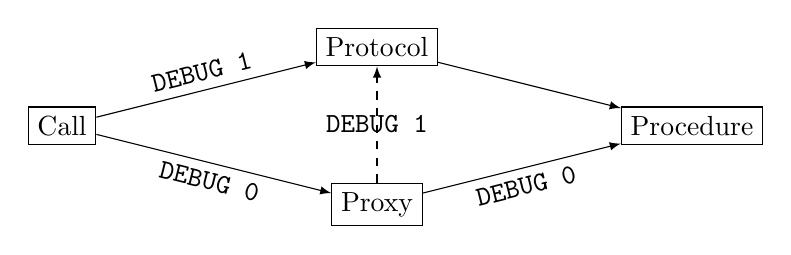
\begin{tikzpicture}

\node[draw, rectangle] (call)      at(0, 0) {Call};
\node[draw, rectangle] (protocol)  at(4, 1) {Protocol};
\node[draw, rectangle] (proxy)     at(4,-1) {Proxy};
\node[draw, rectangle] (procedure) at(8, 0) {Procedure};

\draw[-latex] (call) -- node[above, sloped]{\tt{DEBUG 1}} (protocol);
\draw[-latex] (call) -- node[below, sloped]{\tt{DEBUG 0}} (proxy);

\draw[-latex] (protocol) -- (procedure);

\draw[-latex, dashed] (proxy) -- node{\tt{DEBUG 1}} (protocol);
\draw[-latex] (proxy) -- node[below, sloped]{\tt{DEBUG 0}} (procedure);

\end{tikzpicture}
\end{center}

\note The dashed line signifies that the proxy is essentially a pointer
to the protocol when the method is compiled with \tt{METHOD__} expanding to
\tt{1}, so the dashed line does not incur any additional function call overhead.

Effectively, the protocol can be bypassed only when the caller
and callee (method) jointly agree that debugging is not necessary,
such as when both are compiled with \tt{DEBUG} defined as \tt{0}.
This can be done to reduce code size and improve runtime performance
when the called method has been tested enough times to instill
a reasonable confidence that the code is $possibly$ free of bugs.
However, it is always important to remember that ``\textit{testing shows
the presence, not the absence of bugs}'' (quote by Edsger Wybe Dijkstra);
several classes of bugs cannot be detected using conventional pre-conditions and
post-conditions, and certain bugs manifest only with specific compiler flags.

\pagebreak

\example The following code invokes the method for sorting a list of integers:
when compiled with \tt{DEBUG} as \tt{1}, \tt{CALL__} expands to \tt{1} and the
protocol is invoked, whose name is given by \tt{verifier_(Integers, Sort)}.
With \tt{DEBUG} as \tt{0}, \tt{CALL__} expands to \tt{0}, and the
function pointer \tt{proxy_(Integers, sort)} is used for the invocation.

\code{../compile/sorting.c_}

\note The first argument is later superseded by \tt{.len = length__(&arr_)};
for compiling with \tt{gcc}, the flag \tt{-Wno-override-init-side-effects}
may be required to suppress a warning about non-evaluation of \tt{puts} call.

\exercise The \tt{private} function \tt{burrow} that
implements the recursive merge algorithm uses the signed
type \tt{Ptrdiff} for its parameters accepting index values.
An earlier version of the code used the \tt{Size} type for parameters, which
violated the post-condition in the protocol (when compiled in debugging mode).
On further investigation, the resulting array turned out to be
\tt{4 0 1 2 3 5 6 7 8 9}, which is clearly not sorted.
Stepping through the code then revealed that the array was also being
accessed outside its bounds, one position before the base element.

As a small exercise, try changing the parameter types to
\tt{Size} and observe the results for the same input array.
Find out which part of \tt{burrow} function is affected by
this subtle bug caused by unsigned arithmetic wraparound.
